\documentclass{article}

\usepackage{fancyhdr}
\usepackage{amsmath}
\usepackage{hyperref}
\usepackage{listings}
\usepackage{pdfpages}
\usepackage[margin=1.2in]{geometry}
\lhead{Charles Pehlivanian}
\chead{May 20, 2016}
\rhead{BRFSS Proposal}
\cfoot{\thepage}
\pagestyle{fancy}

\hypersetup{colorlinks=true, urlcolor=blue}

\begin{document}

\title{Simple Cost Model}
\author{Charles Pehlivanian}
\date{May 20, 2016}

\maketitle

\begin{abstract}

A simple trading cost model is specified and fit based on realized trading trajectories of parent orders on exchanges within CMEGroup for clients of Quantitative Brokers. The fit incorporates Spread, Temporary, and Permanent Cost assumptions, although those costs are not explicitly estimated, only aggregate cost. As a next step we would estimate these costs separately, and fit a true intra-order model. The current model is meant to be a first step or proof-of-concept.

\end{abstract}
\section*{Dataset}

The dataset consists of summary statistics for realized child trade confirms by parent order. All trades occur on CME Globex and are classified by the Intrument Codes as given in Table 1.

\begin{table}
\centering
\begin{tabular}{|l|c|c|}
\hline
Inst Code & Description & \#Parent Orders\\
\hline
AG & CBOT Ags & 5724\\
EN & NYMEX Energy & 6957\\
EQ & Equity Index & 8155\\
FX & FX Pairs & 2925\\
IR & Interest Rate & 17760\\
MT & NYMEX Metals & 9169\\
\hline
\hline
TOTAL & & 45690\\
\hline
\end{tabular}
\caption{CME Instrument Code Summary.}
\label{tab:template}
\end{table}

The trade universe consists of the Firm's {\em BOLT} orders, which are arrival-price-benchmarked and attempt to minimize implementation shortfall. See any standard textbook. The remainder of the trades are {\em STROBE} trades which attempt to replicate vwap (or twap, if no volume curve scheduling is used) over the trading window.

Define

\begin{align*}
cost &=& 1e4 * sidesign * (vwap - arrival\textunderscore price)/arrival\textunderscore price\\
pov &=& (parent\textunderscore order\textunderscore participation) * (duration) * (duration\textunderscore wtd\textunderscore volatility)\\
S &=& mid\textunderscore market\textunderscore spread\\
\end{align*}

where

\begin{align*}
vwap &= \frac{1}{\sum_{i=0}^{n}v_i}\sum_{i=0}^{n}p_i v_i\\
arrival\textunderscore price &= \text{midprice at order conception}\\
duration &= \text{length of in sample order in munutes}\\
mid\textunderscore market\textunderscore spread &= \text{avg spread in basis points for underlying market}\\
\end{align*}

etc.

\section*{Model Specification}

The model is a power law in the POV factor, with constant, and spread-based additional summands. After consideration of several models, this was found to give the best fits (see following for basic summary metrics) without sacrificing simplicity. In summary

\begin{align}
Cost = C + \theta S + \beta pov^{\gamma} 
\end{align}

The model fits were carried out in Python using the {\em scipy.ODR} Orthogonal Distance Regression module.

\section*{Fits}

The model fits by Instrument Class follow. The important $\left(\beta , \gamma\right)$  are shown in Table 2., as well as quality of fit graphs - theoretical v empirical. The empirical fit is averaged by bin, where the number of bins (num\_cuts) varies from 10 to 50. The convexity of the empirical cure is evident in these graphs especially at the low-cost end. Residual R-squareds are given for a theoretical linear fit as well as for the power-law fit. These further justify the choice of a sublinear cost function, which can also be justified on theoretical grounds by a no trading-cost arbitrage argument.

\begin{table}
\centering
\begin{tabular}{|l|c|c|}
\hline
Inst Code & Beta & Gamma \\
\hline
AG & 9.5706 & 0.4309 \\
EN & 2.7326 & 0.1087 \\
EQ & 4.0216 & 0.4277 \\
FX & 0.9242 & 0.2169 \\
IR & 0.7273 & 0.2258 \\
MT & 3.6563 & 0.3815\\
\hline
\hline
ALL & 4.266 & 0.3561 \\
\hline
\end{tabular}
\caption{CME Instrument Code Summary.}
\label{tab:template}
\end{table}

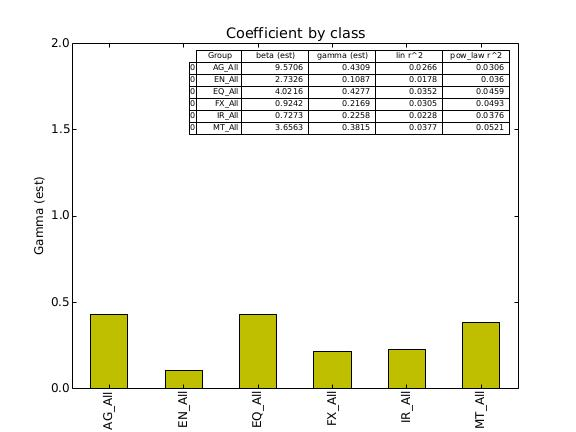
\includegraphics[scale=.74]{./figs/fig1.pdf}

Coefficients by Instrument Class.

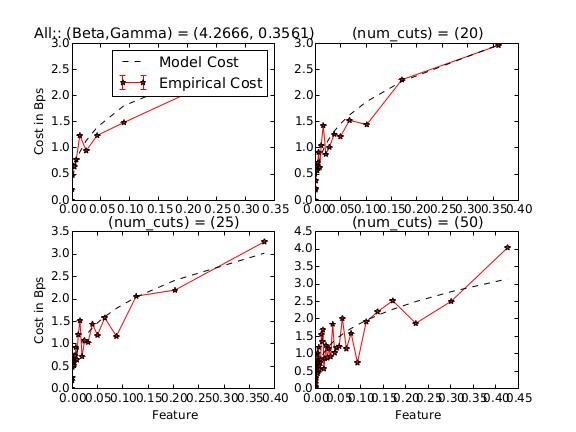
\includegraphics[scale=.74]{./figs//fig2.pdf}

Empirical v Theoretical Plots,, Empirical plots are binned averages.

\section*{Next Steps}
Calibrate intra-order trading cost model.

\bibliographystyle{plain}
\bibliography{bib}

\end{document}
